% {\color{gray}
% Provide descriptions of the deliverables concrete production. It must
% present part of the deliverable (e.g. source code extracts, scientific
% work extracts, \ldots) to illustrate and explain its actual
% production.
% }

The tutorial has been written in Markdown. I decided to go with
Markdown because it is quite easy to use and you can add it to a
GitHub repository.  Considering that we will put this solution onto
GitHub\footnote{See appendix section \ref{app:github}}, this seemed
like a very good idea. This way the tutorial is included with the
solution and is presented nicely. Find more technical information in
the appendix section \ref{app:markdown}.

To begin with, we needed a way to write Markdown files. I used to
write my Markdown files with
ReText\footnote{\url{https://github.com/retext-project/retext}}
however I had a few issues with it and the output did not look all
that nice. I tried switching to Vim, which has a pluggin for
supporting real-time Markdown rendering in a
browser\footnote{\url{https://github.com/suan/vim-instant-markdown}}
but again I had an issue here and it did not even seem to work. I kept
searching a bit more and I found
Remarkable\footnote{\url{https://remarkableapp.github.io/}} which was
pretty good for the purposes of writing the tutorial.

Once we were set for writing the tutorial, we began with writing down
things we already knew how to do. So we build the tutorial as we went,
feeding it with new information as we learnt and discovered it.

Some parts of the tutorial required us to completely restart from
scratch because once you have everything set up, there are things that
differ compared to doing it the first time around. Especially all the
things related to GCP have been done from scratch to show to the user
everything he needs to know to get started. Once everything is set up
there are fewer things to worry about, but they are important to
highlight the first time around.

Markdown has the ability to insert images, so we used it to our
advantage to illustrate a lot of things. See an example of a picture
in figure \ref{fig:markdown}. Furthermore, it allows us to include
references, either external or internal ones. So we can have
references to other websites or to other sections within the file.

We also used this to our advantage, to introduce various other
notions, without interrupting the flow of the text. See figure
\ref{fig:markdown}.

% \begin{figure}
%     \centering
%     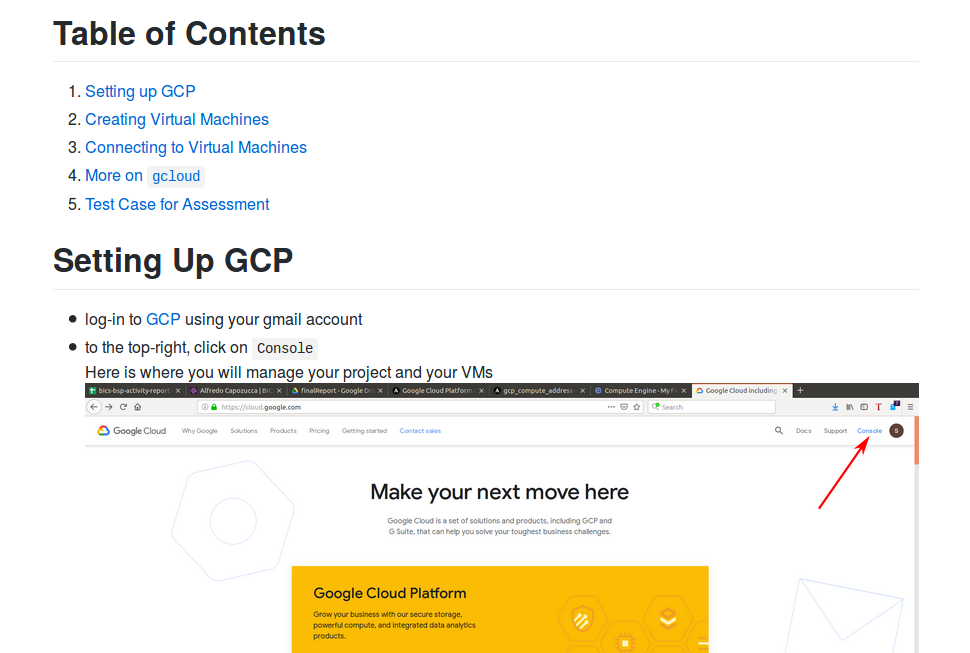
\includegraphics[width=.5\textwidth]{Images/markdown-showcase.png}
%     \caption{Markdown example}
%     \label{fig:markdown}
% \end{figure}

Here we have, for instance, the table of contents which is followed by
a few items colored in blue. This means that you can click on it to
jump some place else. For the table of content, it makes you jump to
the corresponding section in the tutorial. Also, in the first bullet
point in the figure, you can see that \textit{GCP} is colored blue.
This one will actually take you to the Google Cloud Platform.  We used
this all throughout the tutorial to send the reader, in case of need,
to a specific section to get a refresher or some additional
information.
